\subsection{Harder--Narasimhan 滤过}\label{src:9.1.3-subsection}
每个向量丛都以唯一的方式由半稳定向量丛构成: 这称为\newterm{Harder--Narasimhan 滤过}{Harder--Narasimhan filtration}, 有时简称 HN 滤过.
\begin{theorem}[Harder--Narasimhan 滤过]\label{src:9.1.21}
域 $\Bbbk$ 上光滑几何连通射影曲线 $C$ 上的向量丛有唯一的滤过
\[
F_\bullet:0=F_0\subseteq F_1\subseteq F_2\subseteq\cdots\subseteq F_n=F,
\]
使得对每个 $i$, 因子 $F_i/F_{i-1}$ 半稳定, 且
\[
\mu(F_1/F_0)>\mu(F_2/F_1)>\cdots>\mu(F_n/F_{n-1}).
\]
若 $\Bbbk'/\Bbbk$ 是域扩张, 则 $0\subseteq F_1\otimes_{\Bbbk}\Bbbk'\subseteq\cdots\subseteq F_n\otimes_{\Bbbk}\Bbbk'$ 是 $F\otimes_{\Bbbk}\Bbbk'$ 的 Harder--Narasimhan 滤过.
\end{theorem}
\begin{remark}\label{src:9.1.22}
子层 $F_1\subseteq F$ 称为\newterm{最大不稳定化子层}{maximal destabilizing subsheaf}: 它半稳定, 并由下述性质唯一刻画: 对每个子层 $E\subseteq F$, 有 $\mu(F_1)\geq\mu(E)$, 且等号成立当且仅当 $E\subseteq F_1$.
\end{remark}
\begin{remark}\label{src:9.1.23}
若 $C=\mathbb P^1$ 且 $F=\bigoplus_{i=1}^n\mathcal O(d_i)^{\oplus r_i}$, 其中 $d_1>\cdots>d_n$, 则 Harder--Narasimhan 滤过由 $F_j=\bigoplus_{i\leq j}\mathcal O(d_i)^{\oplus r_i}$ 给出, 第 $j$ 个因子 $F_j/F_{j-1}\cong\mathcal O(d_j)^{\oplus r_j}$ 的斜率为 $d_j$.
\end{remark}
\begin{remark}\label{src:9.1.24}
利用映射 $[\mathbb A^1/\mathbb G_m]\to\cBun_{r,d}$ 与向量丛滤过之间的对应 (命题~\bookref{7.9.1}), 向量丛 $F$ 的 Harder--Narasimhan 滤过对应于将 $1$ 映到 $F$ 的唯一映射 $[\mathbb A^1/\mathbb G_m]\to\cBun_{r,d}$.
\end{remark}
\bookfiguretarget{9.1.25}
\begin{figure}[H]
\centering
\begin{tikzpicture}[scale=0.85,>=Stealth]
\coordinate (O) at (0,0);\coordinate (A) at (-1.3,0.2);
\coordinate (B) at (-2.1,1);\coordinate (C) at (-1.8,2);
\coordinate (D) at (-0.9,2.8);\coordinate (E) at (1.3,3.6);
\coordinate (F) at (3.6,3.9);
\draw (-3.15,0)--(4,0) node[right] {$-\deg$};
\draw (0,-0.3)--(0,4.25) node[above] {$\operatorname{rk}$};
\draw[blue!45,line width=2.5pt] (O)--(A)--(B)--(C)--(D)--(E)--(F);
\draw (O)--(A)--(B)--(C)--(D)--(E)--(F)--cycle;
\foreach \P in {A,B,C,D,E,F}{\fill (\P) circle (2pt);}
\node[below] at (-1.3,-0.18) {$Z(F_1)$};\node[left] at (B) {$Z(F_2)$};
\node[above left] at (C) {$Z(F_3)$};\node[above] at (E) {$Z(F_{k-1})$};
\node[right] at (F) {$Z(F)$};
\node[blue,right,fill=white] at (0.2,0.9) {$Z(F_2/F_1)$};
\draw[blue,->] (0.2,0.9) to[bend right=10] (-1.65,0.55);
\node[blue,right,fill=white] at (0.2,2.0) {$Z(F_3/F_2)$};
\draw[blue,->] (0.2,2.0) to[bend right=10] (-1.9,1.5);
\node[blue,above] at (2.55,4.15) {$Z(F/F_{k-1})$};
\draw[blue,->] (2.5,4.15) to[bend right=20] (2.4,3.75);
\end{tikzpicture}
\bookfigurehref{9.1.25}
\caption{用 $Z(F)=-\deg(F)+\operatorname{rk}(F)i$ 表示斜率, Harder--Narasimhan 滤过由 Harder--Narasimhan 多边形确定.}\label{src:9.1.25}
\end{figure}
\begin{proof}
如图~\bookref{9.1.25}, 考虑 $F$ 的\newterm{Harder--Narasimhan 多边形}{Harder--Narasimhan polygon}
\[
\operatorname{HNP}(F):=\{Z(E)\mid E\subseteq F,\ \mu(E)\geq\mu(F)\}\text{ 的凸包}.
\]
由引理~\bookref{9.1.27}, 存在整数 $D$, 使得对所有 $E\subseteq F$, 有 $\deg(E)\leq D$, 因而 $\operatorname{HNP}(F)$ 下有界, 即位于竖直线 $x=-D$ 的右侧. 它还被水平线 $y=\operatorname{rk}(E)$ 从上方限制. 由于 $Z(E)\in\mathbb Z+i\mathbb Z$, $Z(E)$ 的可能取值只有有限个. 所以, $\operatorname{HNP}(F)$ 只有有限个极端点 $z_i$, 每个都可写为某子层 $F_i\subseteq F$ 的 $z_i=Z(F_i)$. 将 $F_i$ 排序, 使得 $\mu(F_1)>\cdots>\mu(F_k)=\mu(F)$, 并令 $F_0=0$. 我们断言
\begin{enumerate}[(a)]
\item $F_{i-1}\subseteq F_i$;
\item $F_i\subseteq F$ 是满足 $z_i=Z(F_i)$ 的唯一子层;
\item $F_i/F_{i-1}$ 半稳定, 且斜率递减: $\mu(F_1/F_0)>\cdots>\mu(F_k/F_{k-1})$.
\end{enumerate}
为证明 (a), 考虑 $F$ 的子层 $F_{i-1}\cap F_i$ 和 $F_{i-1}+F_i$. 短正合列
\[
0\to F_{i-1}\cap F_i\to F_{i-1}\oplus F_i\to F_{i-1}+F_i\to0
\]
蕴含 $Z(F_{i-1}\cap F_i)+Z(F_{i-1}+F_i)=Z(F_{i-1})+Z(F_i)$.
\begin{center}
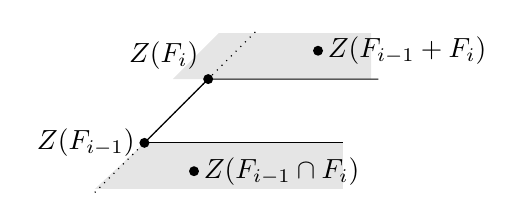
\begin{tikzpicture}[scale=0.9]
\fill[gray!20] (0,-0.65)--(3.5,-0.65)--(3.5,0)--(0.7,0)--cycle;
\fill[gray!20] (1.1,0.9)--(3.9,0.9)--(3.9,1.55)--(1.75,1.55)--cycle;
\draw (0.7,0)--(1.6,0.9)--(4,0.9);\draw (0.7,0)--(3.5,0);
\draw[dotted] (0,-0.7)--(2.3,1.6);
\fill (0.7,0) circle(2pt) node[left] {$Z(F_{i-1})$};
\fill (1.6,0.9) circle(2pt) node[above left] {$Z(F_i)$};
\fill (1.4,-0.4) circle(2pt) node[right] {$Z(F_{i-1}\cap F_i)$};
\fill (3.15,1.3) circle(2pt) node[right] {$Z(F_{i-1}+F_i)$};
\end{tikzpicture}
\end{center}
因为 $F_{i-1}$ 和 $F_i$ 是极端点, $Z(F_{i-1}\cap F_i)$ 位于 $Z(F_{i-1})$ 的右下方, 而 $Z(F_{i-1}+F_i)$ 位于 $Z(F_i)$ 的右上方. 因为 $F_{i-1},F_i$ 是相邻极端点, 只有在 $Z(F_{i-1}\cap F_i)=Z(F_{i-1})$ 且 $Z(F_{i-1}+F_i)=Z(F_i)$ 时才可能发生这种情况. 这蕴含 $F_{i-1}\cap F_i=F_{i-1}$, 即 $F_{i-1}\subseteq F_i$. 相同的论证蕴含 (b): 若子层 $F_i'\subseteq F$ 满足 $Z(F_i')=Z(F_i)$, 则 $F_i'=F_i$. 对 (c), $F_i/F_{i-1}$ 的半稳定性来自 $\operatorname{HNP}(F)$ 的凸性: 若 $E\subseteq F_i/F_{i-1}$ 是不稳定化子层, 则其逆像 $\widetilde E\subseteq F_i$ 位于连接 $Z(F_{i-1})$ 与 $Z(F_i)$ 的线段左侧. 因为 $\mu(F_{i-1})>\mu(F_i)$, 有 $\mu(F_i/F_{i-1})>\mu(F_{i+1}/F_i)$.

唯一性形式地来自凸包极端点的唯一性, 并蕴含此滤过在域扩张下保持不变. 另见 \cite[引理 1.3.7]{HN75}, \cite[命题 5.4.2]{LP97}, \cite[定理 1.3.4]{HL10} 和 \cite[\S2]{Bay11}.
\end{proof}
\begin{corollary}[来自证明]\label{src:9.1.26}
若子层 $E\subseteq F$ 满足 $\mu(E)\geq\mu(F)$, 则 $Z(E)\in\operatorname{HNP}(F)$.
\end{corollary}
\begin{lemma}\label{src:9.1.27}
若 $F$ 是 $C$ 上向量丛, 则存在整数 $D$, 使得对所有子层 $E\subseteq F$, 有 $\deg E\leq D$.
\end{lemma}
\begin{proof}
若 $C=\mathbb P^1$, 则由分类向量丛的 Birkhoff--Grothendieck 定理 (\bookref{9.1.5}) 得到. 否则, 选取有限态射 $f:C\to\mathbb P^1$. 因为 $f$ 平坦, $f_*F$ 是向量丛. 若 $E\subseteq F$ 是子层, 则 $f_*E\subseteq f_*F$ 是子层. 由 Riemann--Roch 定理 (\bookref{9.1.2}), $\chi(E)=\deg(E)+\operatorname{rk}(E)(1-g)$, 所以只需证明 $\chi(E)$ 上有界, 但这由 $\mathbb P^1$ 的情形得到, 因为 $\chi(C,E)=\chi(\mathbb P^1,f_*E)=\deg(f_*E)+\operatorname{rk}(f_*E)$.
\end{proof}
\begin{exercise}[简单, 后文需要]\label{src:9.1.28}
建立上述引理的如下相对版本: 若 $S$ 是 Noether $\Bbbk$-概形, $F$ 是 $C\times S$ 上秩为 $r$, 次数为 $d$ 的向量丛族, 证明存在整数 $D$, 使得对每个 $s\in S$ 和每个子层 $E\subseteq F_s$, 有 $\deg E\leq D$.
\end{exercise}
由于 Harder--Narasimhan 滤过唯一且在域扩张下保持不变, 得到:
\begin{corollary}\label{src:9.1.29}
对域扩张 $\Bbbk'/\Bbbk$, $C$ 上向量丛 $F$ 半稳定, 当且仅当 $F\otimes_{\Bbbk}\Bbbk'$ 在 $C_{\Bbbk'}$ 上半稳定.
\end{corollary}
\begin{exercise}[中等]\label{src:9.1.30}
证明稳定性不满足类似结论.
\end{exercise}
\begin{exercise}\label{src:9.1.31}
对 $C$ 上向量丛 $E$, 以 $\mu_{\max}(E)$ 和 $\mu_{\min}(E)$ 表示 $E$ 的 Harder--Narasimhan 因子的最大与最小斜率. 推广引理~\bookref{9.1.15}(1), 证明若 $C$ 上向量丛 $E,F$ 满足 $\mu_{\min}(E)>\mu_{\max}(F)$, 则 $\Hom_{\mathcal O_C}(E,F)=0$.
\end{exercise}
\subsection{Jordan--H\"older 滤过与 S-等价}\label{src:9.1.4-subsection}
$C$ 上每个半稳定向量丛 $F$ 都有\newterm{Jordan--H\"older 滤过}{Jordan--H\"older filtration} $F_\bullet$, 其因子 $\operatorname{gr}_i:=F_i/F_{i-1}$ 是与 $F$ 斜率相同的稳定向量丛. 虽然此滤过不唯一, 但因子在置换意义下唯一. 将它与 Harder--Narasimhan 滤过结合, 可对每个向量丛作滤过, 使其因子为稳定向量丛.
\begin{proposition}[Jordan--H\"older 滤过]\label{src:9.1.32}
设 $F$ 是 $C$ 上半稳定向量丛. 假设
\[
0=F_0\subseteq F_1\subseteq\cdots\subseteq F_k=F
\quad\text{和}\quad
0=F_0'\subseteq F_1'\subseteq\cdots\subseteq F_\ell'=F
\]
是滤过, 其因子 $\operatorname{gr}_i=F_i/F_{i-1}$ 和 $\operatorname{gr}_i'=F_i'/F_{i-1}'$ 是稳定向量丛, 且 $\mu(F)=\mu(\operatorname{gr}_i)=\mu(\operatorname{gr}_i')$. 则 $\ell=k$, 并存在置换 $\sigma\in\operatorname{Sym}_k$, 使得 $\operatorname{gr}_i\cong\operatorname{gr}_{\sigma(i)}'$.
\end{proposition}
\begin{proof}
给定斜率的半稳定向量丛组成 Abel 范畴 (习题~\bookref{9.1.17}), 其单对象为稳定向量丛. 此命题对 Abel 范畴中任何 Artin 且 Noether 的对象均成立 \cite[Tag 0FCK]{SP}. 证明是一个初等归纳论证, 类似于有限群合成列的存在性证明.
\end{proof}
因此, 下述定义是良定义的.
\begin{definition}[伴随分次]\label{src:9.1.33}
半稳定丛 $F$ 的\newterm{伴随分次}{associated graded} 为
\[
\operatorname{gr}F\cong\bigoplus_i\operatorname{gr}_i,
\]
其中 $\operatorname{gr}_i=F_i/F_{i-1}$ 是相对于任意 Jordan--H\"older 滤过 $0=F_0\subseteq F_1\subseteq\cdots\subseteq F_k$ 的因子.
\end{definition}
\begin{definition}[S-等价]\label{src:9.1.34}
秩与次数相同的两个半稳定向量丛 $E$ 和 $F'$ 称为\newterm{S-等价}{S-equivalent},\footnote{``S-等价''中的``S''指 Seshadri.} 若 $\operatorname{gr}E\cong\operatorname{gr}F$.
\end{definition}
由 Jordan--H\"older 滤过 (\bookref{9.1.32}), 每个半稳定向量丛都与其伴随分次 S-等价. 由命题~\bookref{7.9.1}, 此滤过对应映射 $[\mathbb A^1/\mathbb G_m]\to\cBun_{r,d}^{\mathrm{ss}}$, 将 $1$ 映到 $[F]$, 将 $0$ 映到伴随分次 $\operatorname{gr}F=\bigoplus_iF_i/F_{i-1}$; 后者多重稳定. 虽然多重稳定极限 $\operatorname{gr}F$ 唯一, 但映射 $[\mathbb A^1/\mathbb G_m]\to\cBun_{r,d}^{\mathrm{ss}}$ 并非典范的.

在下述陈述与证明中, 我们将利用 $\mathcal M_{r,d}^{\mathrm{ss}}$ 是有限型代数叠这一事实 (其证明将在后文独立给出, 见定理~\bookref{9.2.8}).
\begin{proposition}\label{src:9.1.35}
设 $\Bbbk$ 是特征为 $0$ 的代数闭域.
\begin{enumerate}[(1)]
\item $C$ 上秩为 $r$, 次数为 $d$ 的向量丛 $F$ 多重稳定, 当且仅当 $[F]\in\cBun_{r,d}^{\mathrm{ss}}$ 为闭点.
\item $C$ 上秩为 $r$, 次数为 $d$ 的两个半稳定向量丛 $F_1,F_2$ S-等价, 当且仅当在 $|\cBun_{r,d}^{\mathrm{ss}}|$ 中, $\overline{\{[F_1]\}}\cap\overline{\{[F_2]\}}\ne\emptyset$.
\end{enumerate}
\end{proposition}
\begin{proof}
对 (1), 若 $F$ 不多重稳定, 则 Jordan--H\"older 滤过 $F_\bullet$ 定义映射 $[\mathbb A^1/\mathbb G_m]\to\cBun_{r,d}^{\mathrm{ss}}$, 将 $1$ 映到 $F$, 将 $0$ 映到 $\operatorname{gr}F$, 这说明 $[F]$ 不是闭点. 另一方面, 若 $F$ 多重稳定而 $[F]$ 不是闭点, 则 $[F]$ 的闭包中存在闭点 $[G]\in\mathcal M_{r,d}^{\mathrm{ss}}$ (由 $\mathcal M_{r,d}^{\mathrm{ss}}$ 的拟紧性), 且 $G\not\cong F$. 由上文, $G$ 必也多重稳定, 特别地, 由推论~\bookref{9.1.16}, $\underline{\operatorname{Aut}}(G)$ 约化, 从而线性约化 (因为 $\operatorname{char}(\Bbbk)=0$!). 由不稳定化定理 (\bookref{8.3.8}), 存在态射 $[\mathbb A^1/\mathbb G_m]\to\cBun_{r,d}$, 将 $1$ 映到 $F$, 将 $0$ 映到 $G$. 由命题~\bookref{7.9.6}, 这对应于伴随分次为 $G$ 的滤过 $0=F_0\subseteq\cdots\subseteq F_n=F$. 因为 $F=\bigoplus_{i\in I}S_i$ 是斜率与 $F$ 相同的稳定向量丛的直和, 每个 $F_i$ 必为某些 $S_i$ 的直和. 这蕴含伴随分次丛 $G$ 同构于 $F$, 矛盾.

对 (2), 若 $F_1,F_2$ S-等价, 则存在伴随分次丛同构的 Jordan--H\"older 滤过 $F_{1,\bullet},F_{2,\bullet}$. 它们对应于映射 $f_1,f_2:[\mathbb A^1/\mathbb G_m]\to\cBun_{r,d}^{\mathrm{ss}}$, 满足 $f_i(1)\simeq F_i$ 且 $f_1(0)\simeq f_2(0)$. 因而 $[F_1]$ 和 $[F_2]$ 在 $\cBun_{r,d}^{\mathrm{ss}}$ 中的闭包有非空交. 反之, 若 $\overline{\{[F_1]\}}\cap\overline{\{[F_2]\}}$ 非空, 则它包含闭点 $[G]\in|\cBun_{r,d}^{\mathrm{ss}}|$, 此点位于 $[F_1]$ 和 $[F_2]$ 的闭包中. 由不稳定化定理 (\bookref{8.3.8}), 存在映射 $f_1,f_2:[\mathbb A^1/\mathbb G_m]\to\cBun^{\mathrm{ss}}$, 满足 $f_i(1)\simeq F_i$ 且 $f_1(0)\simeq f_2(0)\simeq G$. 因为 $G$ 是闭点, $G$ 多重稳定, 与 $f_1,f_2$ 对应的滤过是伴随分次丛同构的 Jordan--H\"older 滤过. 所以 $F_1,F_2$ S-等价.
\end{proof}
一旦建立良模空间 $\pi:\cBun_{r,d}^{\mathrm{ss}}\to M_{r,d}^{\mathrm{ps}}$ 的存在性 (定理~\bookref{9.3.11}), 上述 (2) 蕴含两个向量丛 $F_1,F_2$ S-等价当且仅当 $\pi([F_1])=\pi([F_2])$.
